\def\difficulty{1}
\sujet{Image filtering}

\begin{note}This tutorial work aims to investigate different image filters for smoothing, enhancing or highlighting intensity variations. 
\end{note}

\noindent The different processes will be realized on the following images:
\begin{figure}[h]
\begin{center}
\subfloat[osteoblast cells]{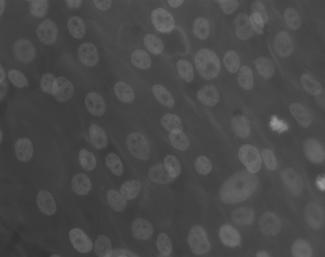
\includegraphics[height=4.5cm]{osteoblaste.jpg}}
\hspace{1cm}
\subfloat[blood cells]{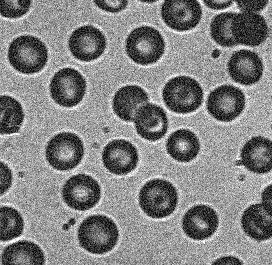
\includegraphics[height=4.5cm]{bloodCells.jpg}}
\end{center}
\end{figure}


\section{Low-pass filtering}
Low-pass filtering aims to smooth the fast intensity variations of the image to be processed.
\begin{itemize}
	\item Test the low-pass filters 'mean', 'median', 'min', 'max' and 'gausian' on the noisy image 'blood cells' with the use of the \matlabregistered{} functions {\tt imfilter} and {\tt nlfilter}.\\
Be careful to the function options for border problems.\\ Also, the \matlabregistered{} function {\tt fspecial} enables an operational window to be generated.
  \item Which filter is suitable for the restoration of this image?
\end{itemize}

%%%%%%%%%%%%%%%%%%%%%%%%%%%%%%%%%%%%%%%%%%%%%%%%%%%%%%%%%%%%%%%%%%%%%%%%%%%%%%%%%%%%%%%%%%%%%%%%%%%
\section{High-pass filtering}
High-pass filtering aims to smooth the low intensity variations of the image to be processed.
\begin{itemize}
	\item Test the high-pass filters $HP$ on the two initial images in the following way: 
	$HP(f)=f-LP(f)$ where $LP$ is a low-pass filtering (see the previous exercise).
	\item[$\bullet$] Test the Laplacian (high-pass) filter on the two initial images with the following convolution mask:
$$
\left[
\begin{array}{ccc}
-1&-1&-1\\
-1&+8&-1\\
-1&-1&-1
\end{array}
\right]
$$
\end{itemize}


\section{Derivative filters}
Derivative filtering aims to detect the edges (contours) of the image to be processed.
\begin{itemize}
	\item
Test the Prewitt and Sobel derivative filters (corresponding to first order derivatives) on the image 'blood cells' with the use of the following convolution masks:
$$
\left[
\begin{array}{ccc}
-1&0&+1\\
-1&0&+1\\
-1&0&+1
\end{array}
\right]
\left[
\begin{array}{rrr}
-1&-1&-1\\
0&0&0\\
+1&+1&+1
\end{array}
\right]
\left[
\begin{array}{ccc}
-1&0&+1\\
-2&0&+2\\
-1&0&+1
\end{array}
\right]
\left[
\begin{array}{rrr}
-1&-2&-1\\
0&0&0\\
+1&+2&+1
\end{array}
\right]
$$
\item Look at the results for the different gradient directions.
\item Define an operator taking into account the horizontal and vertical directions.
\end{itemize}
Remark : the edges could be also detected with the zero-cressings of the Laplacian filtering  (corresponding to second order derivatives)


\section{Enhancement filtering}
Enhancement filtering aims to enhance the contrast or accentuate some specific image characteristics.
\begin{itemize}
	\item[$\bullet$] Test the enhancement filter $E$ on the image 'osteoblast cells' defined as:
	$E(f)=f+HP(f)$ where $HP$ is a Laplacian filter (see exercise 2).
	\item[$\bullet$] Parameterize the previous filter as:
	$E(f)=\alpha f+HP(f)$, or $\alpha\in\mathbb{R}$.
\end{itemize}

\section{Open question}
Find an image filter for enhancing the gray level range of the image 'osteoblast cells'.

